\chapter{Исследовательская часть}

В данном разеделе будут приведены примеры работы программы, а также проведен сравнительный анализ процессорного времени работы реализаций алгоритмов при различных ситуациях на основе полученных данных.

\section{Технические характеристики}

Технические характеристики устройства, на котором выполнялся эксперимент представлены далее:

\begin{itemize}
	\item операционная система --- Ubuntu 22.04.3 \cite{ubuntu} Linux x86\_64;
	\item память --- 16 Гб;
	\item процессор --- Intel® Core™ i5-1135G7 @ 2.40 ГГц.
\end{itemize}

При эксперименте ноутбук не был включен в сеть электропитания.

\section{Демонстрация работы программы}

На рисунке \ref{fig:example} представлен результат работы программы, на котором выводится меню и выполняется каждая из 3 сортировок на предварительно подготовленном массиве чисел.

\begin{figure}[h!]
	\centering
	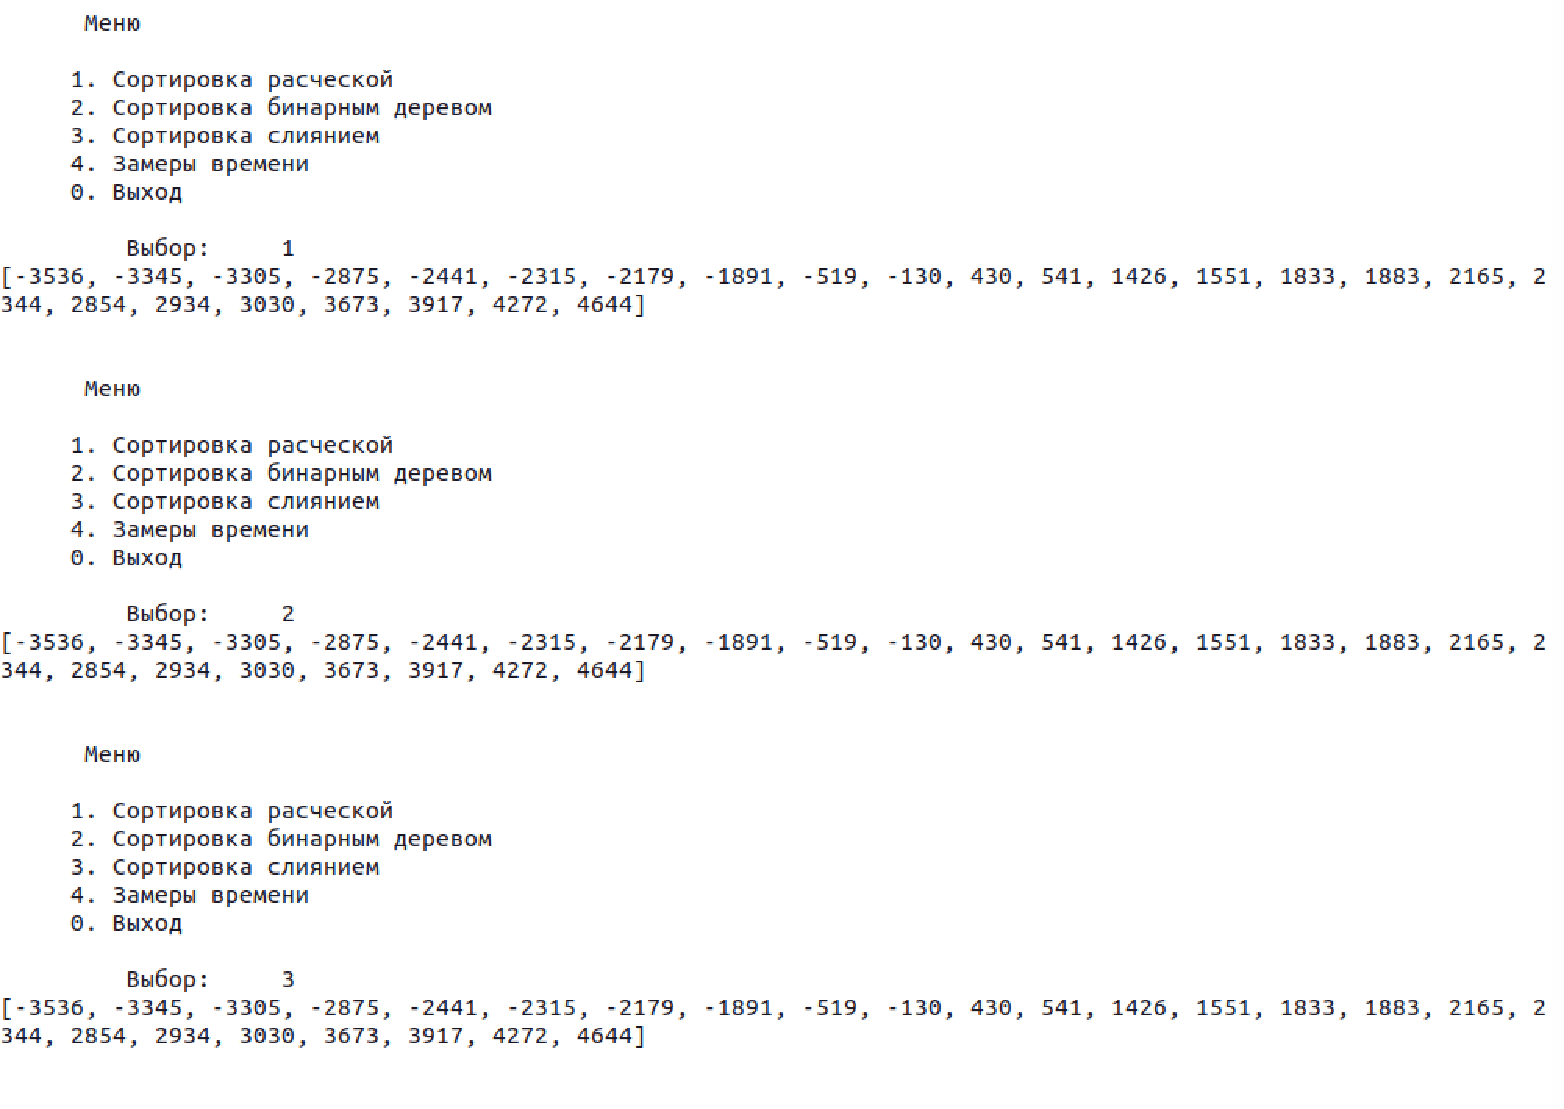
\includegraphics[width=\linewidth]{img/example}
	\caption{Пример работы программы}
	\label{fig:example}
\end{figure}
\clearpage

\section{Время выполнения алгоритмов}

Как было сказано выше, используется функция замера процессорного времени process\_time(...) из библиотеки time на Python. Функция возвращает пользовательское процессорное временя типа float.

Функция используется дважды: перед началом выполнения алгоритма и после завершения, затем из конечного времени вычитается начальное, чтобы получить результат.

Результаты замеров приведены в таблицах \ref{tbl:best}-\ref{tbl:random} (время в мс).

\begin{table}[h]
	\begin{center}
		\begin{threeparttable}
		\captionsetup{singlelinecheck=off, justification=raggedright}
		\caption{Отсортированные данные}
		\label{tbl:best}
		\begin{tabular}{|c|r|r|r|}
			\hline
			Размер & Расческой & Бинарным деревом & Слиянием \\
			\hline
			  100 & 96.68 & 555.99 & 95.46 \\ 
			\hline
			200 & 220.52 & \multicolumn{1}{|r|}{2,263.25} & 222.92 \\ 
			\hline
			300 & 417.48 & \multicolumn{1}{|r|}{5,007.74} & 349.33 \\ 
			\hline
			400 & 577.89 & \multicolumn{1}{|r|}{8,962.32} & 471.86 \\ 
			\hline
			500 & 794.07 & \multicolumn{1}{|r|}{14,073.85} & 604.17 \\ 
			\hline
			600 & 984.98 & \multicolumn{1}{|r|}{20,987.65} & 802.39 \\ 
			\hline
			700 & \multicolumn{1}{|r|}{1,286.17} & \multicolumn{1}{|r|}{29,853.94} & 938.30 \\ 
			\hline
			800 & \multicolumn{1}{|r|}{1,486.94} & \multicolumn{1}{|r|}{38,480.89} & \multicolumn{1}{|r|}{1,073.84} \\ 
			\hline
			900 & \multicolumn{1}{|r|}{1,774.24} & \multicolumn{1}{|r|}{49,576.84} & \multicolumn{1}{|r|}{1,199.23} \\ 
			\hline
		\end{tabular}
		\end{threeparttable}
    \end{center}
\end{table}

\begin{table}[h]
	\begin{center}
		\begin{threeparttable}
		\captionsetup{singlelinecheck=off, justification=raggedright}
		\caption{Отсортированные в обратном порядке данные}
		\label{tbl:worth}
		\begin{tabular}{|c|r|r|r|}
			\hline
			 Размер & Расческой & Бинарным деревом & Слиянием \\
			\hline
			  100 & 102.80 & 557.37 & 105.87 \\ 
			\hline
			200 & 231.22 & 2,224.29 & 224.09 \\ 
			\hline
			300 & 445.14 & 5,045.33 & 352.55 \\ 
			\hline
			400 & 601.85 & 9,001.34 & 463.68 \\ 
			\hline
			500 & 810.16 & 14,074.22 & 606.80 \\ 
			\hline
			600 & 1,045.80 & 20,323.24 & 764.61 \\ 
			\hline
			700 & 1,282.02 & 27,838.25 & 907.07 \\ 
			\hline
			800 & 1,473.24 & 39,628.49 & 1,161.71 \\ 
			\hline
			900 & 1,888.61 & 50,180.55 & 1,242.45 \\ 
			\hline
		\end{tabular}
		\end{threeparttable}
    \end{center}
\end{table}

\begin{table}[h]
	\begin{center}
		\begin{threeparttable}
		\captionsetup{singlelinecheck=off, justification=raggedright}
		\caption{Случайные данные}
		\label{tbl:random}
		\begin{tabular}{|c|r|r|r|}
			\hline
			 Размер & Расческой & Бинарным деревом & Слиянием \\
			\hline
			  100 & 108.12 & 99.93 & 107.90 \\ 
			\hline
			200 & 255.87 & 253.64 & 249.29 \\ 
			\hline
			300 & 470.66 & 400.53 & 400.66 \\ 
			\hline
			400 & 678.91 & 585.54 & 539.63 \\ 
			\hline
			500 & 922.55 & 763.61 & 690.55 \\ 
			\hline
			600 & 1,110.81 & 935.66 & 856.70 \\ 
			\hline
			700 & 1,370.43 & 1,202.98 & 1,016.88 \\ 
			\hline
			800 & 1,576.80 & 1,398.82 & 1,181.66 \\ 
			\hline
			900 & 1,864.26 & 1,618.94 & 1,371.91 \\ 
			\hline
		\end{tabular}
		\end{threeparttable}
    \end{center}
\end{table}

Также на рисунках \ref{fig:sort}-\ref{fig:rand} приведены графические результаты замеров работы реализации сортировок в зависимости от размера входного массива.

\begin{figure}
	\centering
	\includegraphics[width=0.8\linewidth]{img/sort}
	\caption{Отсортированный массив}
	\label{fig:sort}
\end{figure}

\begin{figure}
	\centering
	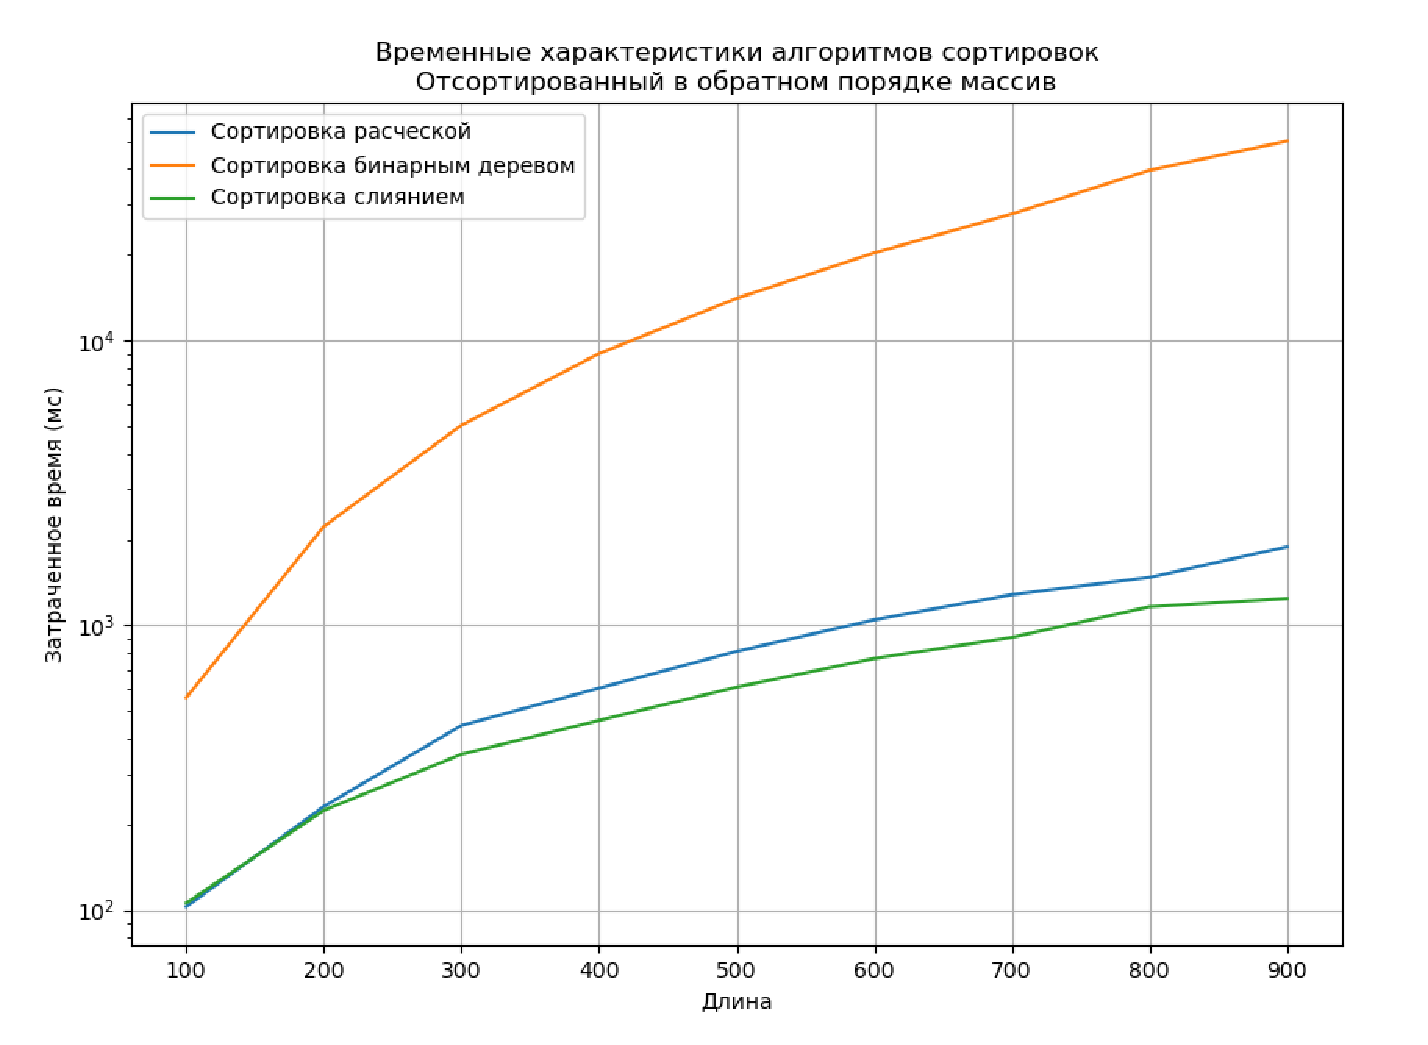
\includegraphics[width=0.8\linewidth]{img/sort_back}
	\caption{Отсортированный в обратном порядке массив}
	\label{fig:sort_back}
\end{figure}

\begin{figure}[h!]
	\centering
	\includegraphics[width=0.8\linewidth]{img/rand}
	\caption{Случайный массив}
	\label{fig:rand}
\end{figure}


\section*{Вывод}
Исходя из полученных результатов, сортировка бинарным деревом при массиве заполненном отсортированными в любом порядке данными работает дольше других примерно в 15 раз, но на случайных значениях она примерно в 1.13 раз медленнее, чем сортировка расческой и в 1.2 раза быстрее сортировки слиянием.
Так же из эксперимента видно, что сортировка слиянием показала себя лучше всех при размере массива более 200 на любых данных, а при отсортированных в прямом и обратном порядках данных она быстрее, чем сортировка расческой примерно в 1.3 раза.
